%%%%%%%%%%%%%%%%%%%%%%%%%%%%%%%%%%%%%%%%%%%%%%%%%%%%
\chapter{Konzept}
\label{sec:Konzept}
%%%%%%%%%%%%%%%%%%%%%%%%%%%%%%%%%%%%%%%%%%%%%%%%%%%%
\todo{einleiten}

\section{Konzeptuelles Design}
Zunächst muss geklärt werden, was dargestellt werden soll bevor entschieden wird, wie es dargestellt wird. \todo{besser formulieren}
\begin{figure}[htbp]
\centering
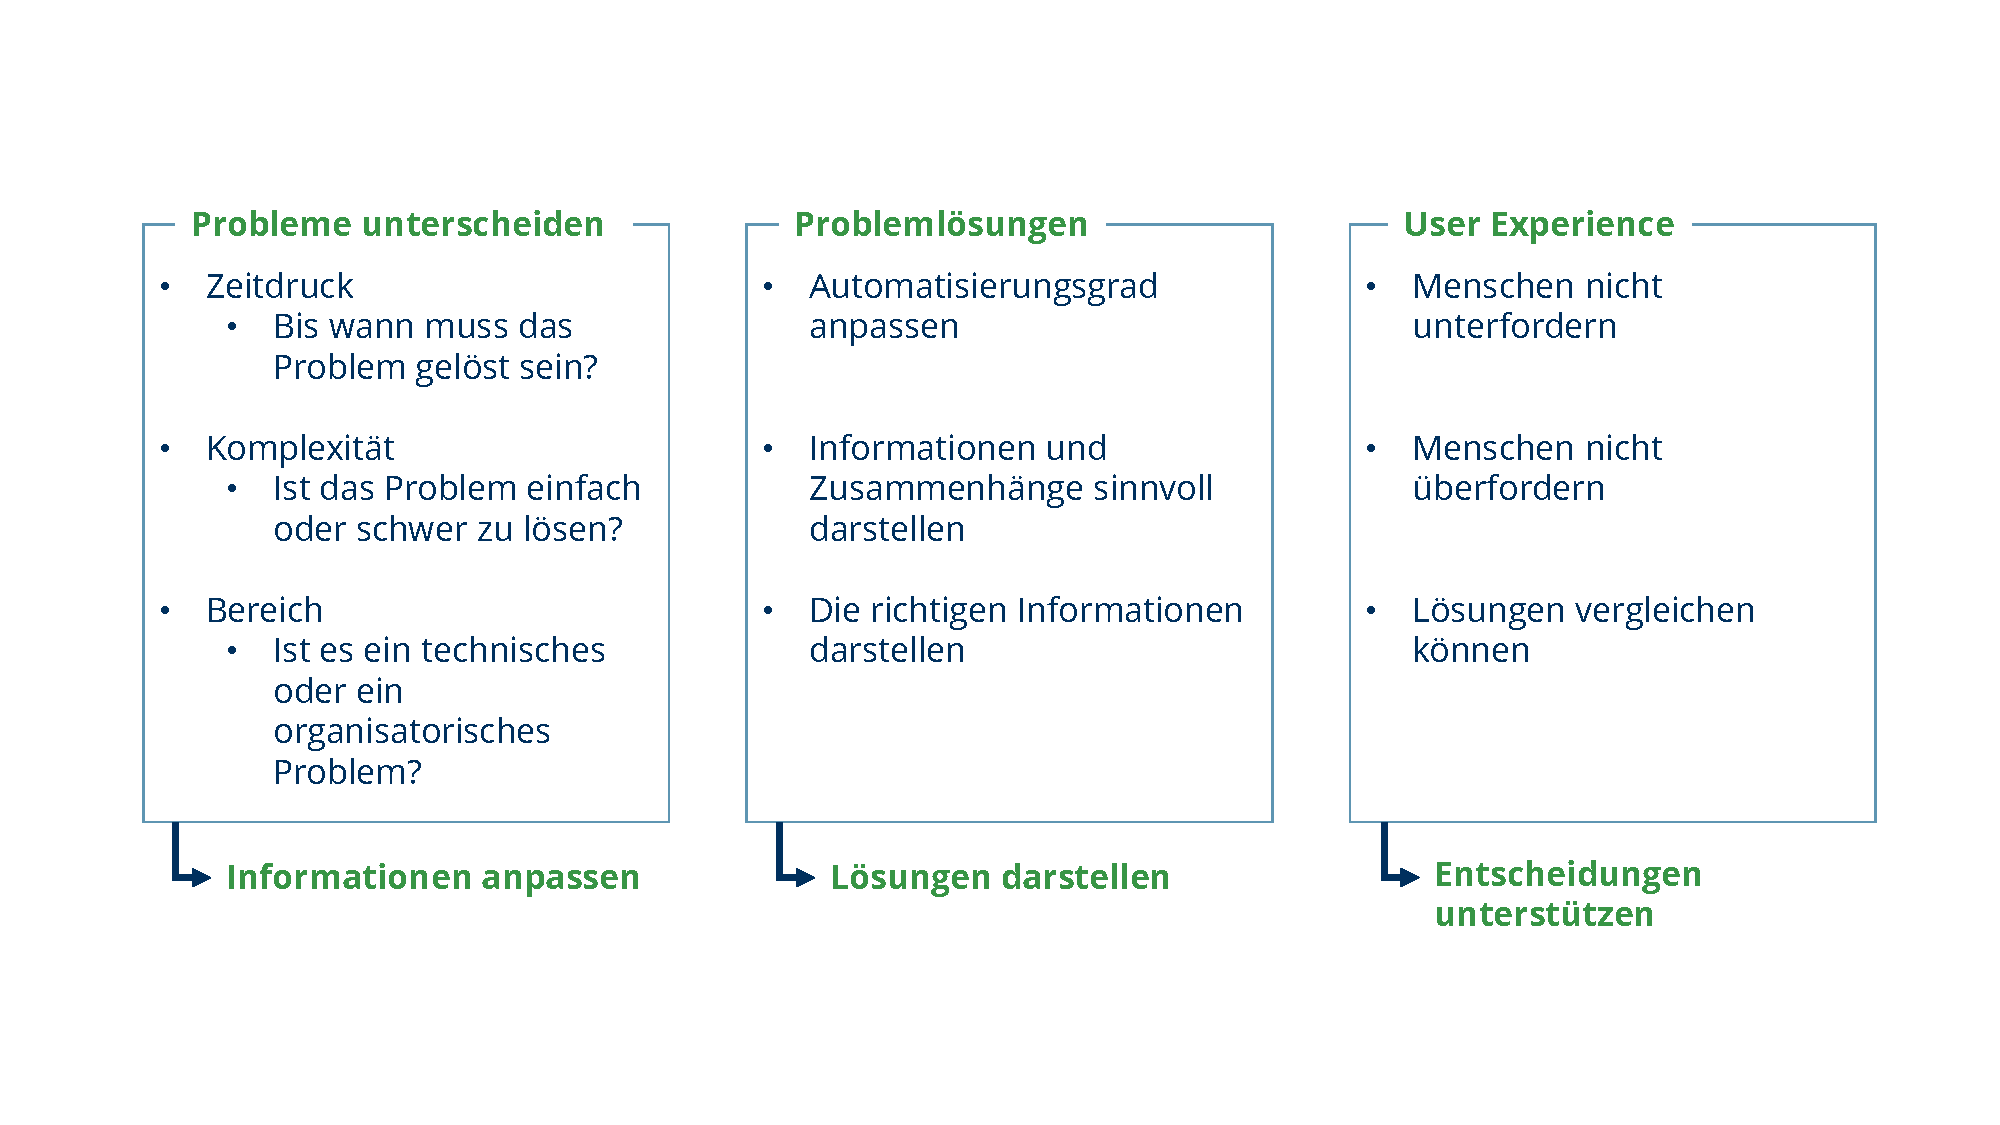
\includegraphics[scale=0.45]{DA_files/Bilder/Konzept/Nutzer-unterstuetzen.pdf}
\caption{•}
\label{pic:Nutzer-Unterstuetzen}
\end{figure}
\\ \\
In Abschnitt \ref{2:Unterscheidung-Probleme} ist bereits aufgeführt, dass sich \textbf{Probleme unterscheiden}. Die Informationen sollen sich entsprechend dem Zeitdruck, der Komplexität des Problems und dem umfassenden Bereich automatisch anpassen. Dadurch soll sowohl eine Unterforderung, als auch eine Überforderung des Menschen verhindert werden.

Die \textbf{Lösungen für das Problem} sollen sinnvoll dargestellt werden. Dabei wird der Autonomiegrad anhand des Zeitdrucks angepasst. Die Menge an dargestellten Informationen und deren Zusammenhänge orientieren sich an der Komplexität des Problems. Die Komplexität des Problems lässt sich aus der Menge an Zusammenhängen ableiten. Deshalb ist es umso wichtiger diese strukturiert und klar darzustellen. Abhängig vom Bereich des Problems sind die richtigen Informationen darzustellen.

Mit einer guten \textbf{User Experience} soll die Entscheidung des Menschen unterstützt werden. Dieser soll mittels geeignetem Autonomiegrad nicht unterfordert werden. Durch die angemessene Darstellung der Informationen ist eine Überforderung zu vermeiden. Die Darstellung der Informationen hängt auch mit der Vergleichbarkeit der Lösungen zusammen. Gibt es mehrere Lösungen, so muss der Nutzer Unterschiede gut erkennen können, um eine geeignete Entscheidung zu treffen.
\\ \\
Wie kann nun der Nutzer durch den Problemlöseprozess begleitet werden? In Abschnitt \ref{2:Phasen-Problemloesen} sind die Phasen des Problemlösens beschrieben. Angelehnt daran wird folgender Ablauf mit entsprechender Unterstützung durch das Assistenzsystem vorgesehen (siehe Bild \ref{pic:Konzeptidee}).
\begin{figure}[htbp]
\centering
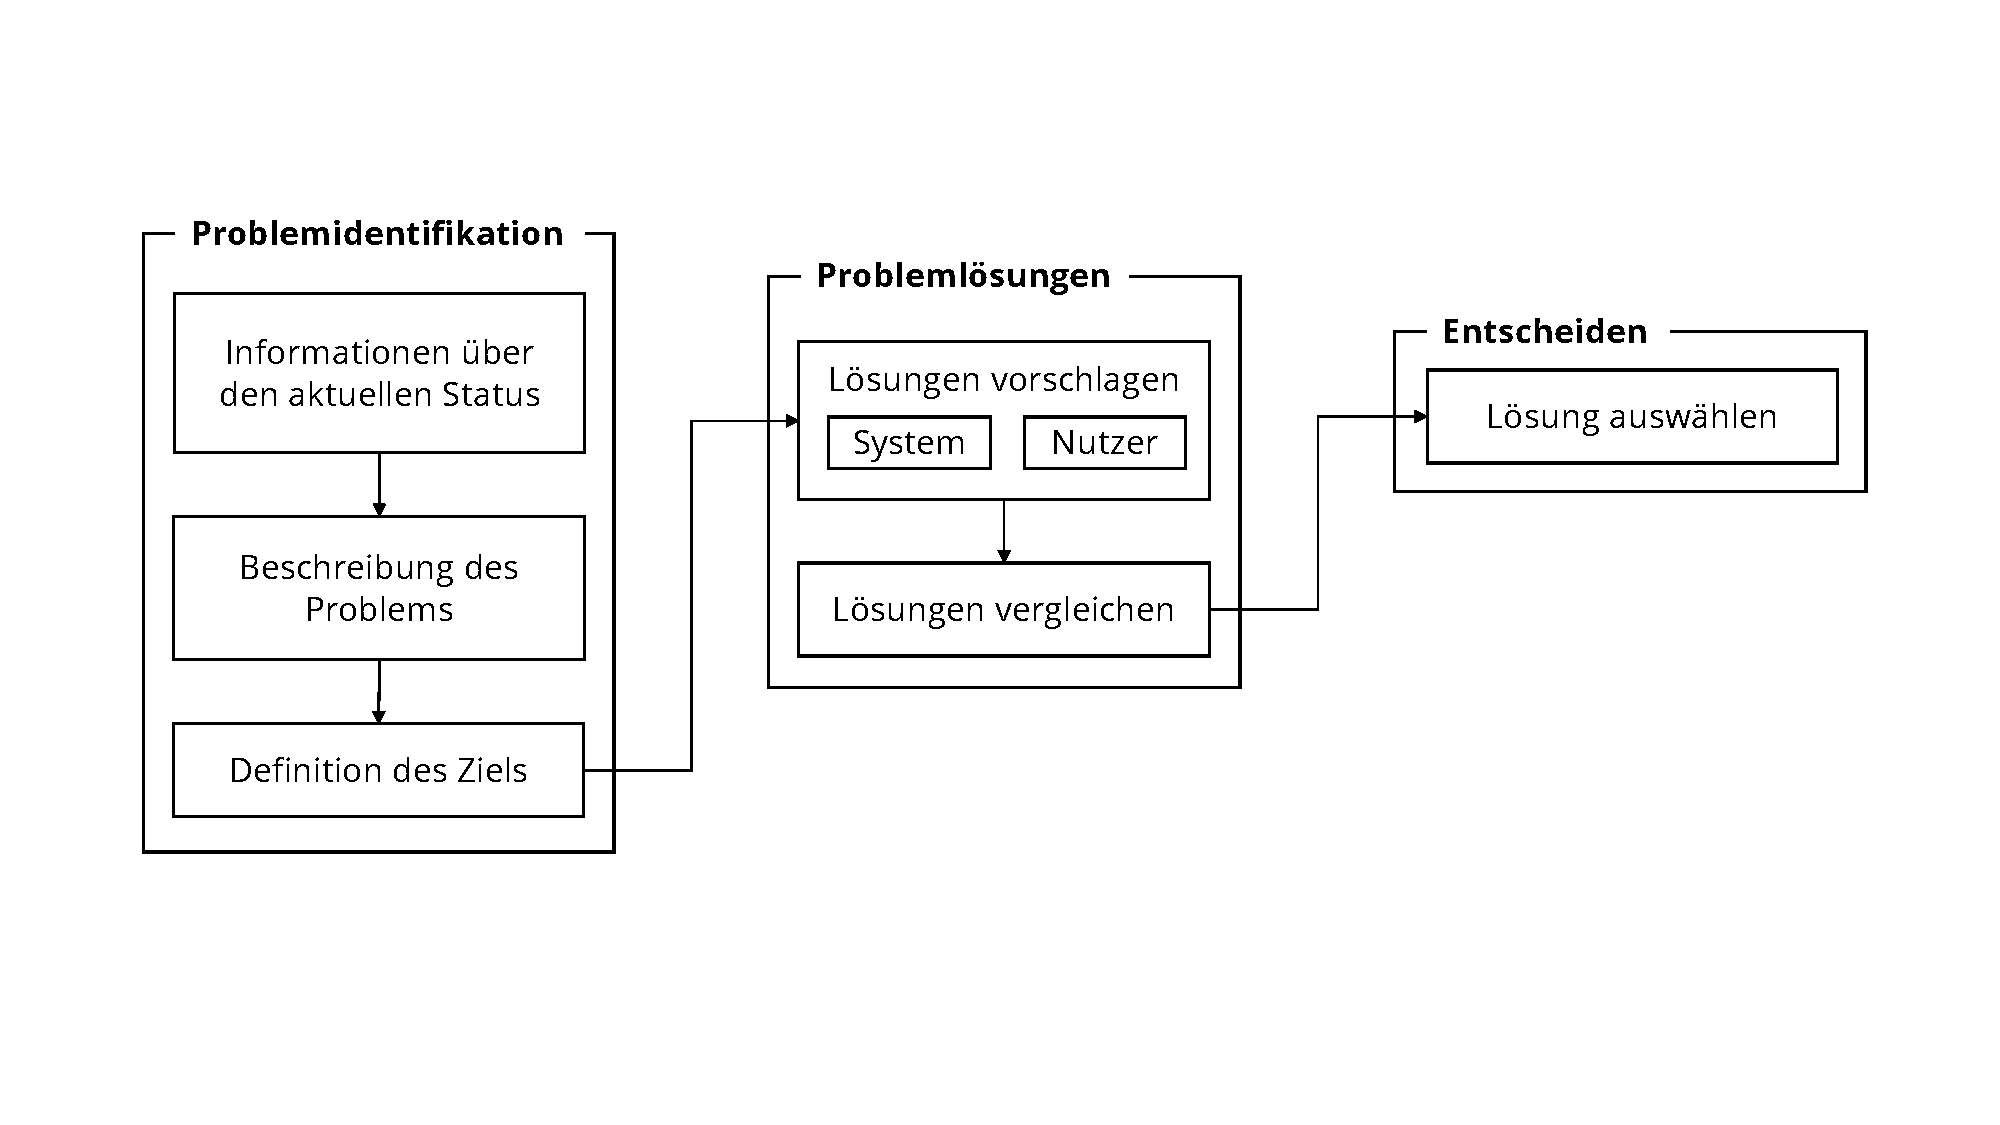
\includegraphics[scale=0.45]{DA_files/Bilder/Konzept/Konzeptidee.pdf}
\caption{Die Schritte des Problemlöseprozess}
\label{pic:Konzeptidee}
\end{figure}

Zunächst muss das Problem identifiziert werden. Dazu stehen dem Nutzer alle Informationen über den aktuellen Status der modularen Anlage zur Verfügung. Durch Meldungen, Warnungen und Alarme können Probleme vom System ausgelöst werden. Weiterführend ist es denkbar, das auch der Nutzer ein Problem definiert. Ist das Problem identifiziert, so muss das Ziel definiert werden. Im Fall eines zu wartenden Moduls kann ein maximaler Produktionsausfall und die dadurch entstehenden Kosten angegeben werden.

Ist das Problem identifiziert und das Ziel definiert, so müssen die möglichen Lösungen betrachtet werden. Lösungen können sowohl vom System als auch vom Nutzer vorgeschlagen werden. Nach Bestimmung der Lösungen erfolgt ein Vergleich dieser. Um eine Entscheidung treffen zu können ist eine Bewertung der verschiedenen Lösungen möglich.

Die Entscheidung wird unterstützt, indem sich die Kriterien und deren Relevanz festlegen lassen. Anhand dieser können die Lösungen gefiltert und die Beste ausgewählt werden.

\subsection{Funktionen}
\todo{einleitenden Text schreiben}
welche Funktionen müssen realisiert werden?

Nach Lösungen und Ursachen suchen

\subsubsection*{Aktueller Status}
Der aktuelle Status kann über die PFE abgelesen werden. Diese gibt einen Überblick über die aktuelle Verschaltung der Module, das Rezept, die Key Performace Indicator (KPIs) und die Services. Auch eine Übersicht über das Anlagenequipment eines jeden Moduls ist vorhanden. Die notwendigen Meldungen, Warnungen und Alarme werden derzeit nicht angezeigt. Durch die Integration dieser kann der Nutzer bei der Problemidentifikation unterstützt werden. Tritt beispielsweise eine Meldung auf, hat der Nutzer die Möglichkeit dieses als Problem aufzunehmen und nach Lösungen zu suchen.

\subsubsection*{Neues Problem}
Hat sich der Nutzer dem Problem angenommen, kann dieses durch Ziele näher spezifiziert werden. Welche grundlegenden Ziele für das Unternehmen relevant sind, kann vorab festgelegt werden. In Bild \ref{pic:Produktionsprozesse-Zielgroessen} sind mögliche Ziele aufgeführt. Für das aktuelle Problem können die relevanten Ziele ausgewählt und genauer spezifiziert werden. \todo{welche Ziele?}

Neben der Beschreibung der Ziele ist es dem Nutzer möglich eine Übersicht über den Problembereich zu erhalten. Dazu markiert das Assistenzsystem zunächst den Bereich in dem das Problem ausgelöst wurde und die zugehörigen Komponenten. Betrifft der Bereich ein bestimmtes Modul, dann werden die zugehörigen Services und der zugehörige Bereich im Rezept markiert. Betrifft der Bereich einen Service, sind die Parameterabhängigkeiten und das zugehörige Equipment relevant. Ausgehend von dem markierten Bereich und geleitet durch die Ziele können Lösungen gefunden werden.

\subsubsection*{Lösungen suchen }
Wie die konkrete Lösung für ein Problem aussieht ist nicht vorherbestimmt. Das Assistenzsystem kann anhand der definierten Ziele Vorschläge liefern. Diese können durch den Nutzer angepasst und bewertet werden. Hier ist der Mensch klar im Vorteil, da dieser Optionen abwägen kann. Des weiteren hat der Nutzer die Möglichkeit selber nach Lösungen zu suchen. Ihm stehen dazu alle Informationen über die Anlage zur Verfügung. Das Assistenzsystem markiert die Veränderungen, die durch die Lösungen entstehen. Dadurch kann der Nutzer den Aufwand abschätzen und bewerten, ob die Lösung gut oder schlecht ist.

\subsubsection*{Lösungen vergleichen}
In vielen Fällen gibt es nicht nur eine richtige Lösung, sondern mehrere Lösungsmöglichkeiten, die gegeneinander abgewogen werden müssen. Dem Nutzer werden dazu die Unterschiede zwischen den Lösungen aufgezeigt. Diese können rein zahlenmäßig sein, wie entstehende Kosten oder der Energieverbrauch eines Moduls. Es ist jedoch auch möglich, dass sich Lösungen strukturell unterscheiden, z.B. anhand der zur Verfügung gestellten Dienste.

\subsubsection*{Entscheiden}
Gibt es mehrere Lösungen, dann muss sich der Nutzer bei einem erfolgreichen Problemlöseprozess für eine entscheiden. \todo{formulieren}

\subsection{Anpassungen}
welche Elemente beeinflussen sich gegenseitig?

Wie wählt das Assistenzsystem Lösungen aus?

Da sich sowohl Probleme, als auch Lösungen von Fall zu Fall unterscheiden, müssen dementsprechend Anpassungen vorgenommen werden. In Abschnitt \ref{3:Anpassung-Aufgabe} ist bereits erwähnt, dass sich die Informationen an das Problem und die Ziele anpassen sollten. Im Zuge dessen sind vor allem die gegenseitigen Abhängigkeiten relevant, auf die im weiteren Verlauf näher eingegangen wird. Damit sich das Assistenzsystem anpassen kann muss identifiziert werden, wo das Problem entstanden ist. Es lassen sich folgende Fälle unterscheiden:
\begin{itemize}
\item \textbf{Modul:} Das gesamte Modul hat ein Problem verursacht.
\item \textbf{Service:} Ein Service hat eine Warnung oder Alarm ausgelöst.
\item \textbf{Rezept:} Das Rezept ist an einer bestimmten Stelle hängen geblieben und kann nicht weiter abgearbeitet werden.
\item \textbf{KPI:} Die KPI weisen Unregelmäßigkeiten auf oder erreichen vorher definierte Grenzwerte.
\end{itemize}

\subsubsection*{Modul}
Ein einzelnes Modul ist sehr eigenständig, da es grundsätzlich auch alleine betrieben werden kann. In der Navigation der PFE ist ersichtlich mit welchen anderen Modulen es verbunden ist. Um eine Problemlösung auf Modulebene zu unterstützen ist es notwendig die zugehörigen Services und den Bereich im Rezept zu markieren. Dadurch kann der Nutzer die Abhängigkeiten erkennen. 

\subsubsection*{Services}
Die Services weisen eine Vielzahl an Abhängigkeiten auf. So kann ein Service direkt mit anderen Services gekoppelt sein (vgl. Abschnitt x) oder durch Parameter eines anderen Services gestartet werden. Diese Kopplung ist auch modulübergreifend möglich. Löst nun ein Service ein Problem aus, werden die abhängigen Services markiert. Dies erleichtert dem Nutzer die Eingrenzung des Problembereichs. Bei der Suche nach Ursachen, warum der Service nicht funktioniert muss es dem Nutzer möglich sein alle Möglichkeiten in Erwägung zu ziehen. So steht dem Nutzer die Möglichkeit zur Verfügung das zugehörige Equipment zum Service anzusehen.

\subsubsection*{Rezept}
Wird das Rezept automatisch ausgeführt besteht die Möglichkeit, dass dieses aufgrund eines Fehlers nicht vollständig ausgeführt werden kann. In so einem Fall wird dem Nutzer angezeigt an welcher Stelle das Rezept abgebrochen wurde und welcher Service zugehörig ist. Ausgehend von der Position im Rezept können die notwendigen Bedingungen überprüft und mögliche Ursachen in Erwägung gezogen werden. Ist die Ursache identifiziert können mit Hilfe des Assistenzsystems Lösungen gefunden werden. So ist es dem Nutzer möglich Veränderung an der entsprechenden Stelle im Rezept vorzunehmen. Diese können dann vom Assistenzsysteme virtuell geprüft werden. Auf diese Weise entsteht eine kollaborative Problemlösung.

\subsubsection*{KPI}
Die Key Performace Indicator beinhalten Kennzahlen \todo{ausformulieren}


\section{Physikalisches Design}
Das physikalische Design beschreibt die konkrete Darstellung der Funktionen und Informationen.

\subsection{Problem beschreiben}


\subsection{Markierung des Bereichs}
